\section{Meshing}\label{sec:meshing}

The mesh in FEM model is the collection of small discrete elements that make up the model geometry or domain.
Meshing is the process of generating a mesh.
Meshing is one of the most important aspects of FEM modeling as the mesh directly influences the accuracy of the solution; it is important that the various gradients are resolved by the mesh.
However, designing a good mesh can be challenging as a finer mesh has a higher computational cost.
A good mesh designer must constantly balance accuracy and computational costs by considering where a mesh can be finer and where it can be coarser.\par

The most fundamental unit of the mesh is the element(s) that comprise the mesh.
There are many different types of elements that can be used for meshing and choosing which ones to use depend primarily on the spatial dimensionality of the model, the particularities of the geometry, and the physics that we wish to model.
Obviously different element types are by necessity needed to model a 2D vs. 3D geometry; you cannot mesh a 3D geometry with 2D squares.\par

\begin{figure}[htb!]
  \centering
  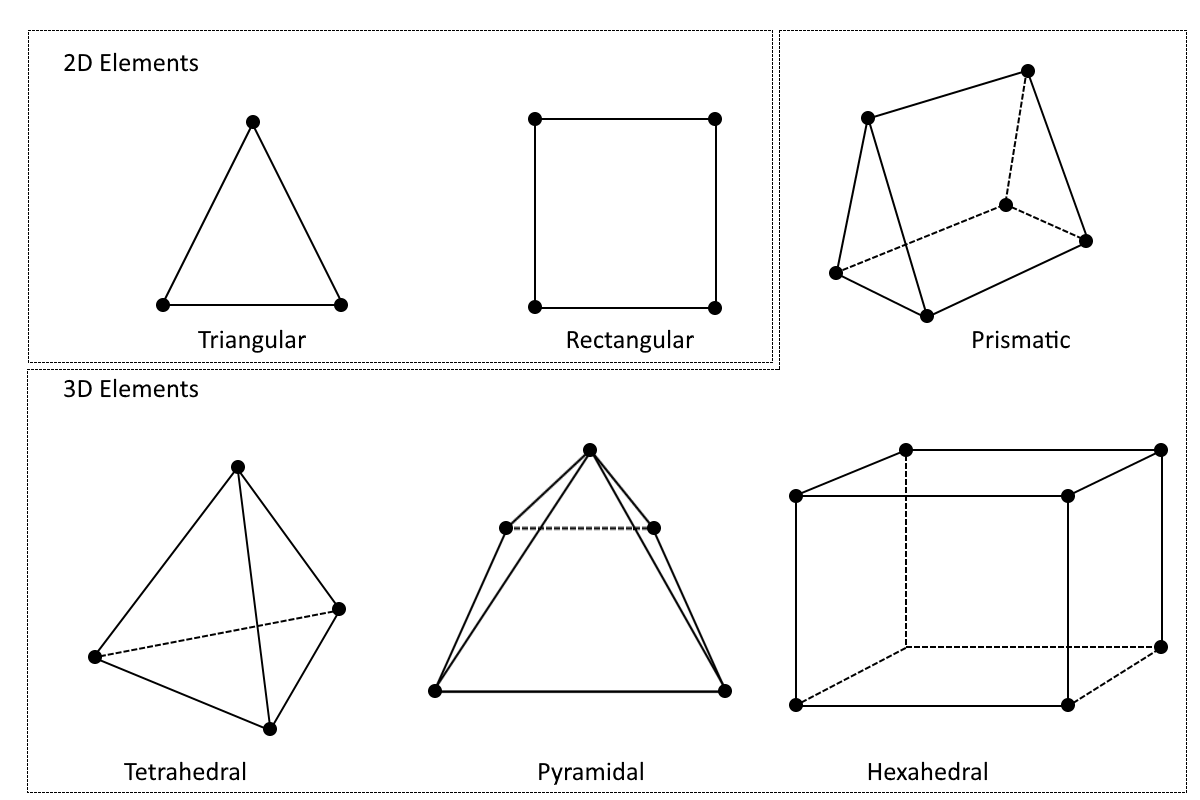
\includegraphics[width=0.75\textwidth]{mesh_elements.png}
  \caption{Some common mesh elements. Figure from COMSOL\cite{noauthor_detailed_nodate}.}
  \label{fig:mesh_elements}
\end{figure}

There are primarily four types of 3D mesh elements available - the tetrahedral, cuboid, prism, and pyramid.
Figure \ref{fig:mesh_elements} shows some common mesh elements.
These can be combined in various ways to represent any 3D geometry.
The most general 3D element is the tetrahedral and will approximate any geometry well.
However, it is not always the most effective choice for meshing a geometry and another element type may be better suited.
This is easiest illustrated with an example.\par

Imagine that you are trying to simulate the laminar flow of some fluid in a pipe.
Because of symmetry, only a wedge of the pipe needs to be explicitly modeled.
Therefore, in this scenario, it might be beneficial to use prism elements rather than tetrahedrals, since these are already wedge shaped.

The laminar pipe flow will have a gradient in the direction of the flow.
Thus the mesh mostly only needs to be fine in the flow direction, while the mesh can be coarser in the radial direction.
Constructing a mesh on this basis would allow us to achieve a solution of high accuracy while still keeping the number of elements relatively small - all through clever mesh design (see Figure \ref{fig:cylinder_mesh}).\par

\begin{figure}[htb!]
  \centering
  \begin{subfigure}{0.49\textwidth}
    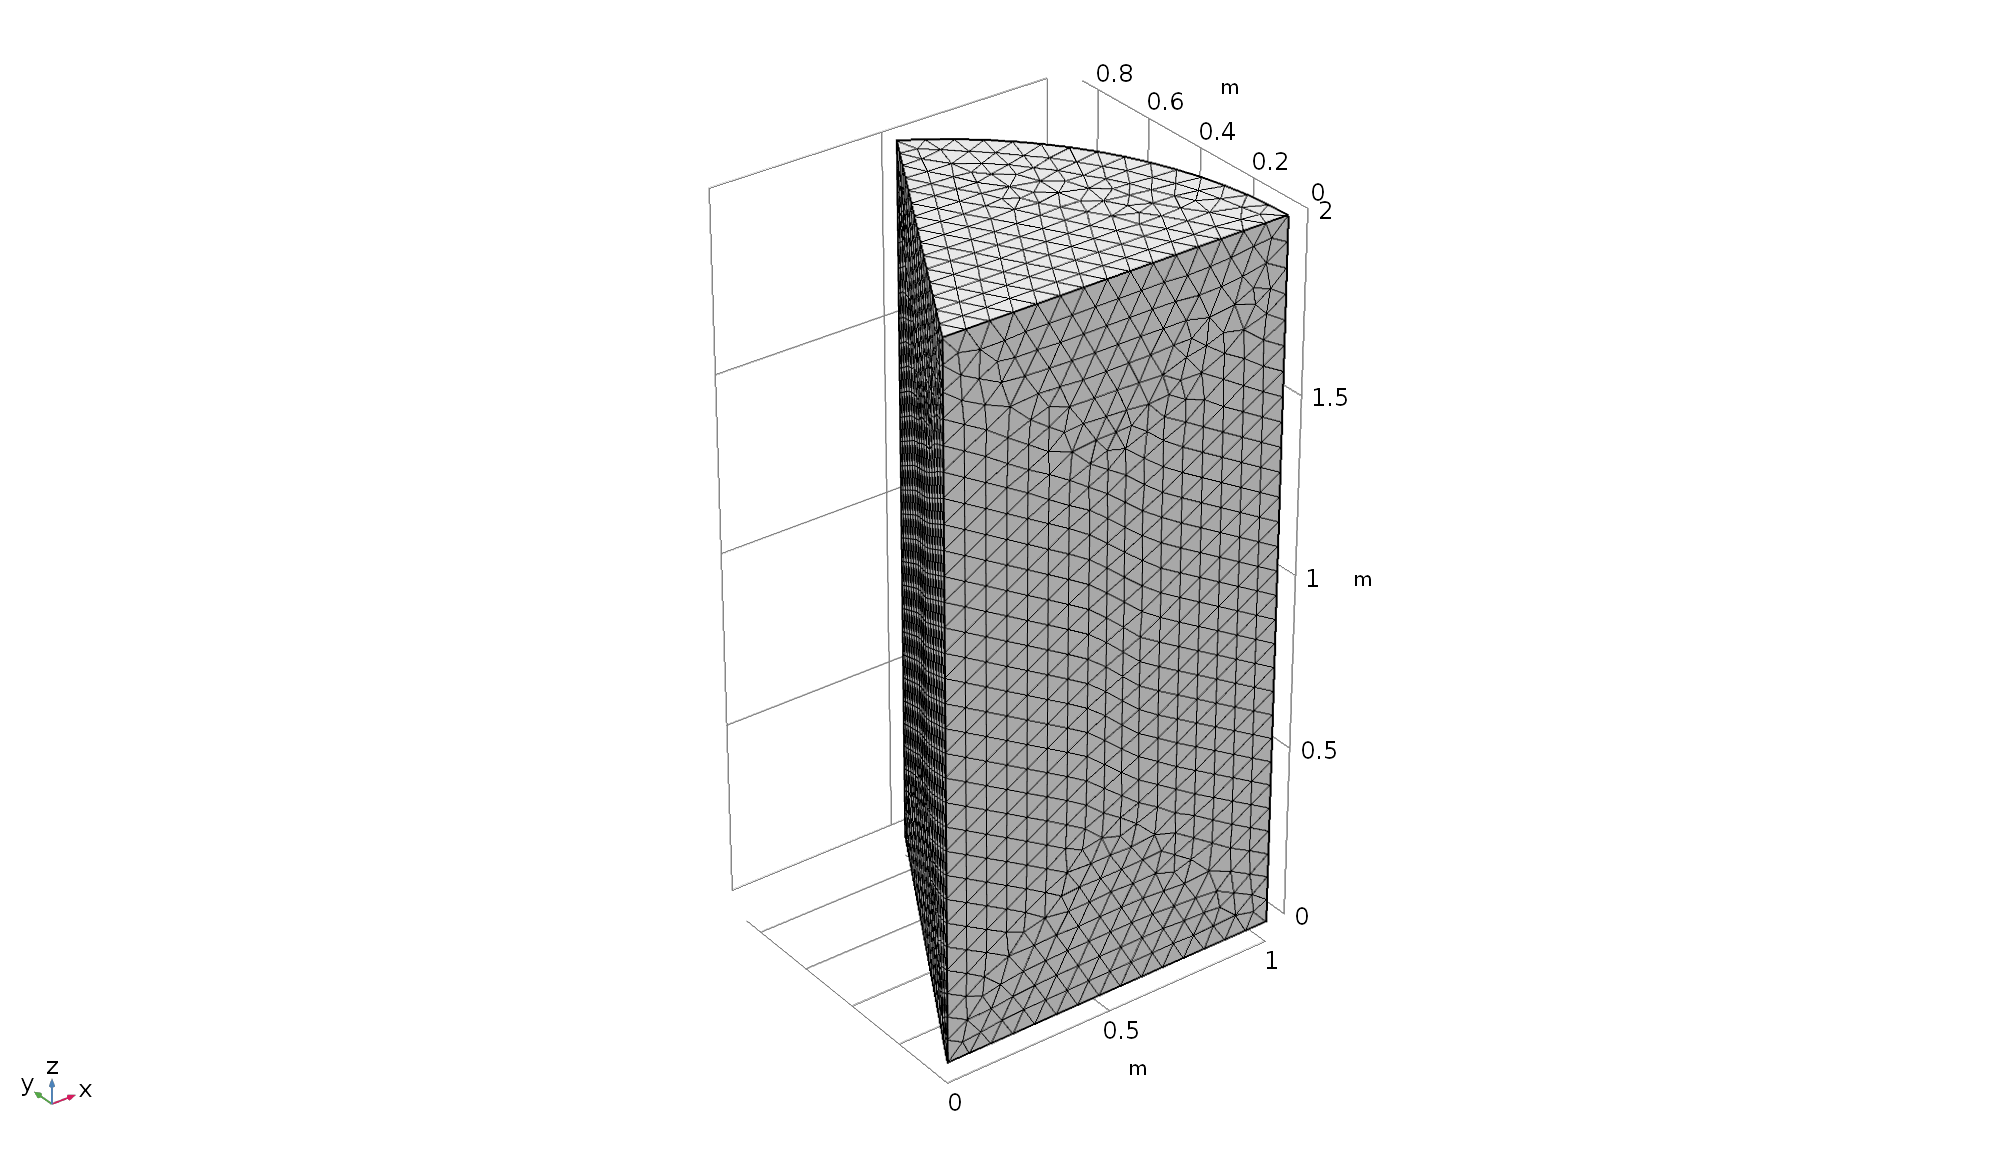
\includegraphics[width=\textwidth]{cylinder_regular_mesh.png}
  \caption{Mesh using tetrahedrals. 50,197 elements.}
  \end{subfigure}
  \begin{subfigure}{0.49\textwidth}
    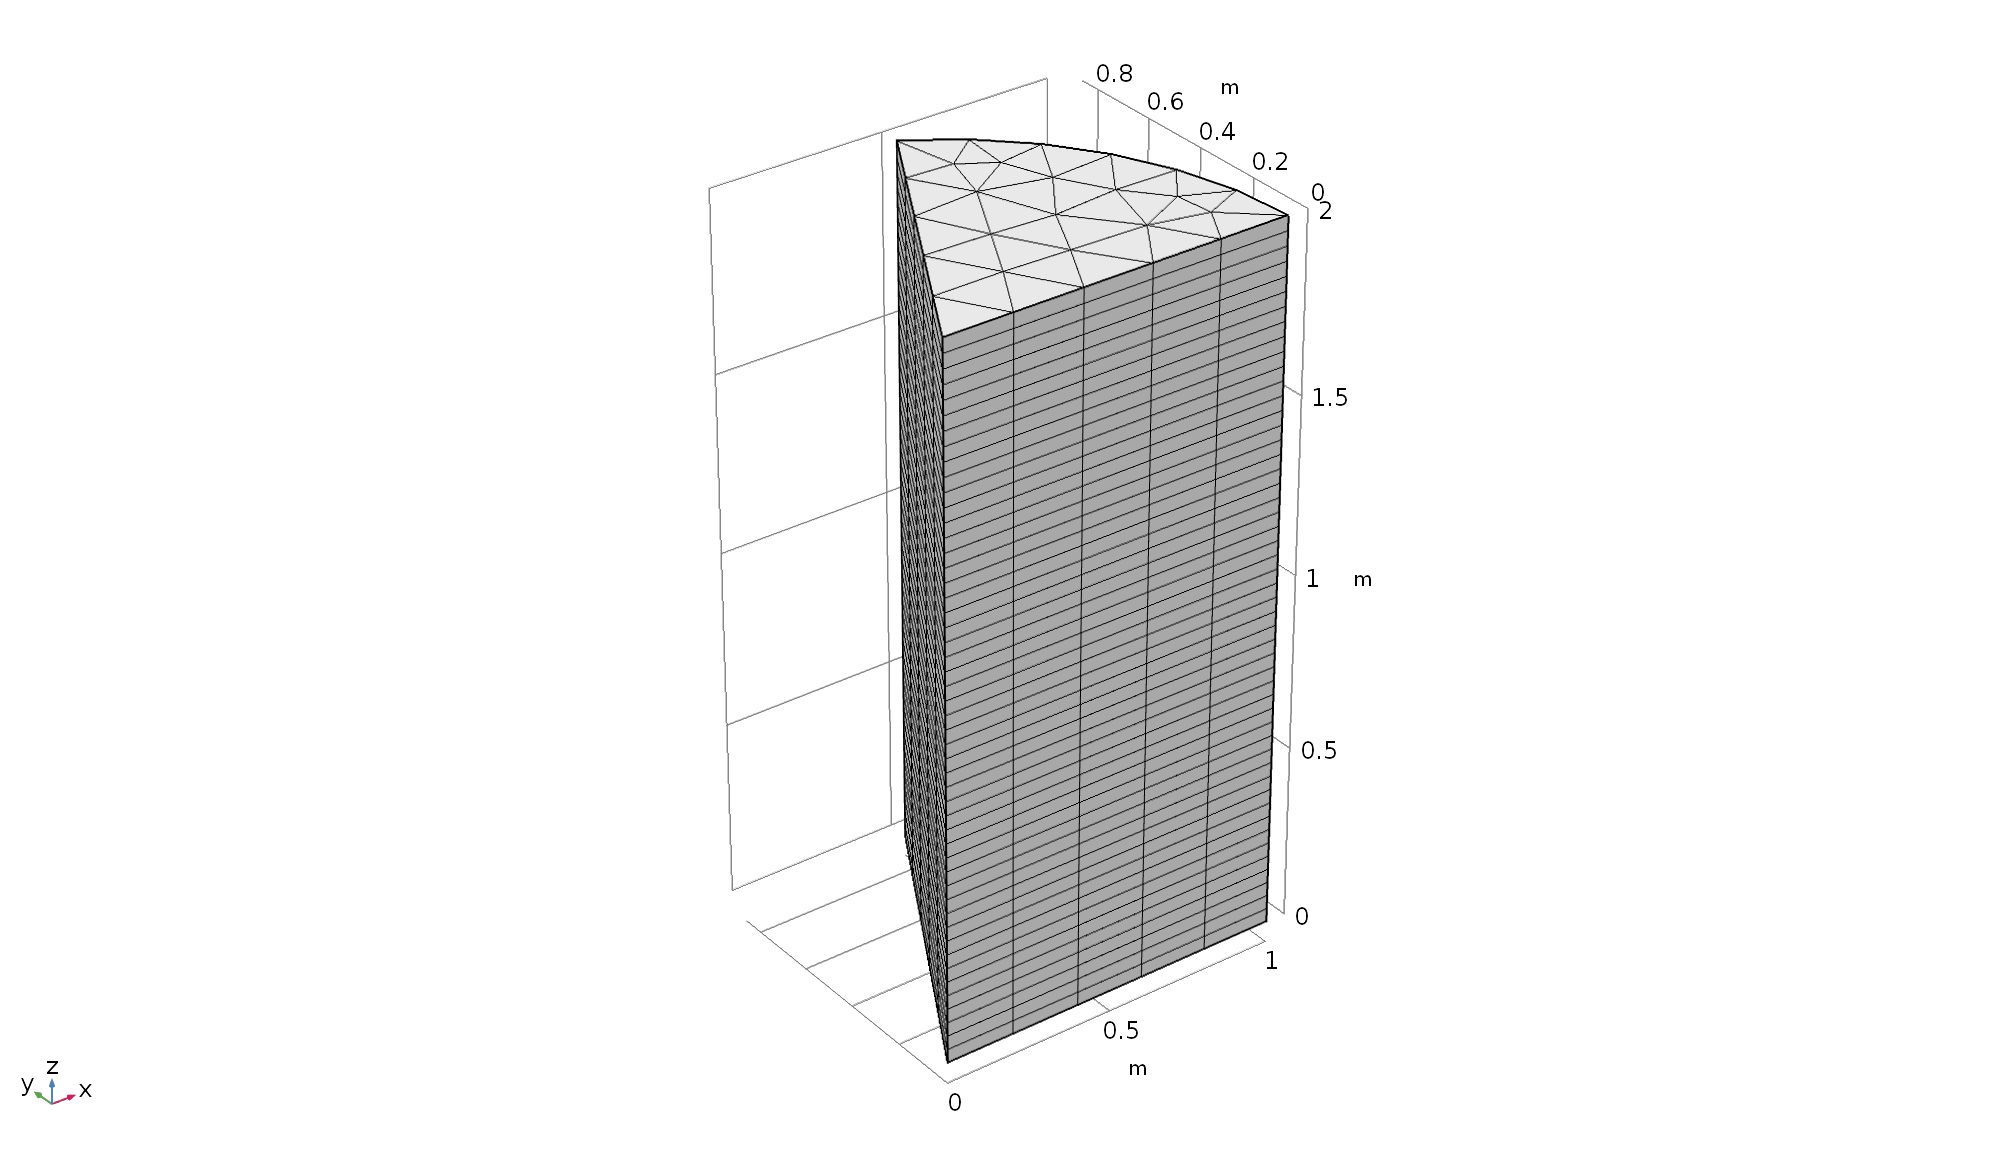
\includegraphics[width=\textwidth]{cylinder_swept_mesh.png}
  \caption{Mesh using prism elements. 1900 elements.}
  \end{subfigure}
  \caption[Example of how physical mesh design can reduce the number of elements.]{By understanding the physics, here considering laminar flow in a pipe (segment), clever mesh design can significantly reduce the number of mesh elements. Notice that the mesh density in the axial direction is more or less the same.}
  \label{fig:cylinder_mesh}
\end{figure}

This is of course a relatively simple example and more complicated geometries may need all kinds of element for constructing a clever design.
These type of multi-element meshes can give significant computational saving but at the expense of often requiring significant user input to be generated.
Sticking to one type of elements is often simpler as these can quickly and easily mesh geometries.\par

Meshing can be done manually, but is often performed by a meshing algorithm.
The creation of these algorithms is a science in itself, but their use often involve passing some basic parameters to the algorithm.
Here the user could, for instance, specify the maximum and minimum element sizes, maximum element growth rate, how finely small features or curves (typically quite difficult to mesh) should be meshed.
These instructions can be specific to various parts of the model, e.g. much finer meshing resolution can be specified for an area of interest and vice versa.
There are also a variety of specialty mesh features such as a mesh boundary layer available: adding finely spaced mesh layers along a boundary.
How to use all of these tools effectively to mesh a geometry is why meshing can be one of the most challenging aspects of FEM modeling.\par

\subsection{Meshing The VI Model}

The first choice we need to make is which type of element to use, and in order to do that we need to think about the gradients of the dependent variables.\par

From van Genuchten's retention curves, we know there will be a large soil moisture gradient in the capillary zone, which will need a relatively fine mesh to be resolved.
The airflow from Darcy's Law will forming some sort of arcing streamline from the ground surface to the foundation crack; the pressure gradient will be inline with these streamline.
The concentration gradient is difficult to predict a priori, but there likely will be some gradient from the groundwater to the ground surface and foundation crack.
Since many of these gradients intersect and go in different directions from each other it makes sense to use tetrahedral elements to mesh the geometry; these are the more general 3D elements.\par

Properly meshing our geometry can be a challenge due to the great range of geometric scale.
The house and soil domains are on the order of meters while the foundation crack is only \SI{1}{\centi\meter} side, and requires very fine meshing.
This is not only due to its small size, but because the contaminant entry will be calculated based on the solution here, which largely determines the indoor contaminant concentration.\par

The COMSOL meshing algorithm only require a few parameters to relatively mesh a geometry with tetrahedrals.
A description of each parameter and its value can be seen in Table \ref{tbl:meshing}.
\begin{table}[htb!]
  \begin{tabularx}{\linewidth}{l c X}
    \toprule
    Input & Value & Description \\
    \midrule
    Maximum element size & \SI{1.5}{\metre} & Maximum size of a element \\
    Minimum element size & \SI{1}{\milli\metre} & Minimum size of a element \\
    Maximum element growth rate & 1.3 & Maximum allowed size increase of adjacent elements. 1.3 indicates that an element can only be 30\% larger than its neighbor. A smaller value gives a finer mesh. \\
    Curvature factor & 0.4 & Ratio between the boundary element size and the geometry curvature radius. A smaller value gives a finer mesh. \\
    Resolution of narrow regions & 1 & Control the number of layers of elements that are created in narrow regions. A larger value gives a finer mesh. \\
    \bottomrule
  \end{tabularx}
  \caption{Inputs to COMSOLs meshing algorithm.}
  \label{tbl:meshing}
\end{table}

\subsection{Boundary Layer Mesh}

When posed with steep gradients in one particular direction at boundaries, as we have here, it is often useful to use a \textit{boundary layer mesh} at the impacted boundaries.
This is a type of mesh that introduces a dense layer of meshes along the normal direction from a boundary.
Boundary layer meshes are common features in meshing algorithms, and COMSOL's is no exception.\par

The number of boundary layers are supplied by the user, and in our case we will use 8 layers, but more could be added if needed.
The distance between each layer is determined by the size of the other elements in its vicinity, as well as the distance growth rate between each layer, which we set to 1.3, i.e. the distance increases by 30\% for each layer.
Figure \ref{fig:mesh} shows our completed mesh.\par

\begin{figure}[htb!]
  \centering
  \begin{subfigure}[b]{\textwidth}
    \centering
    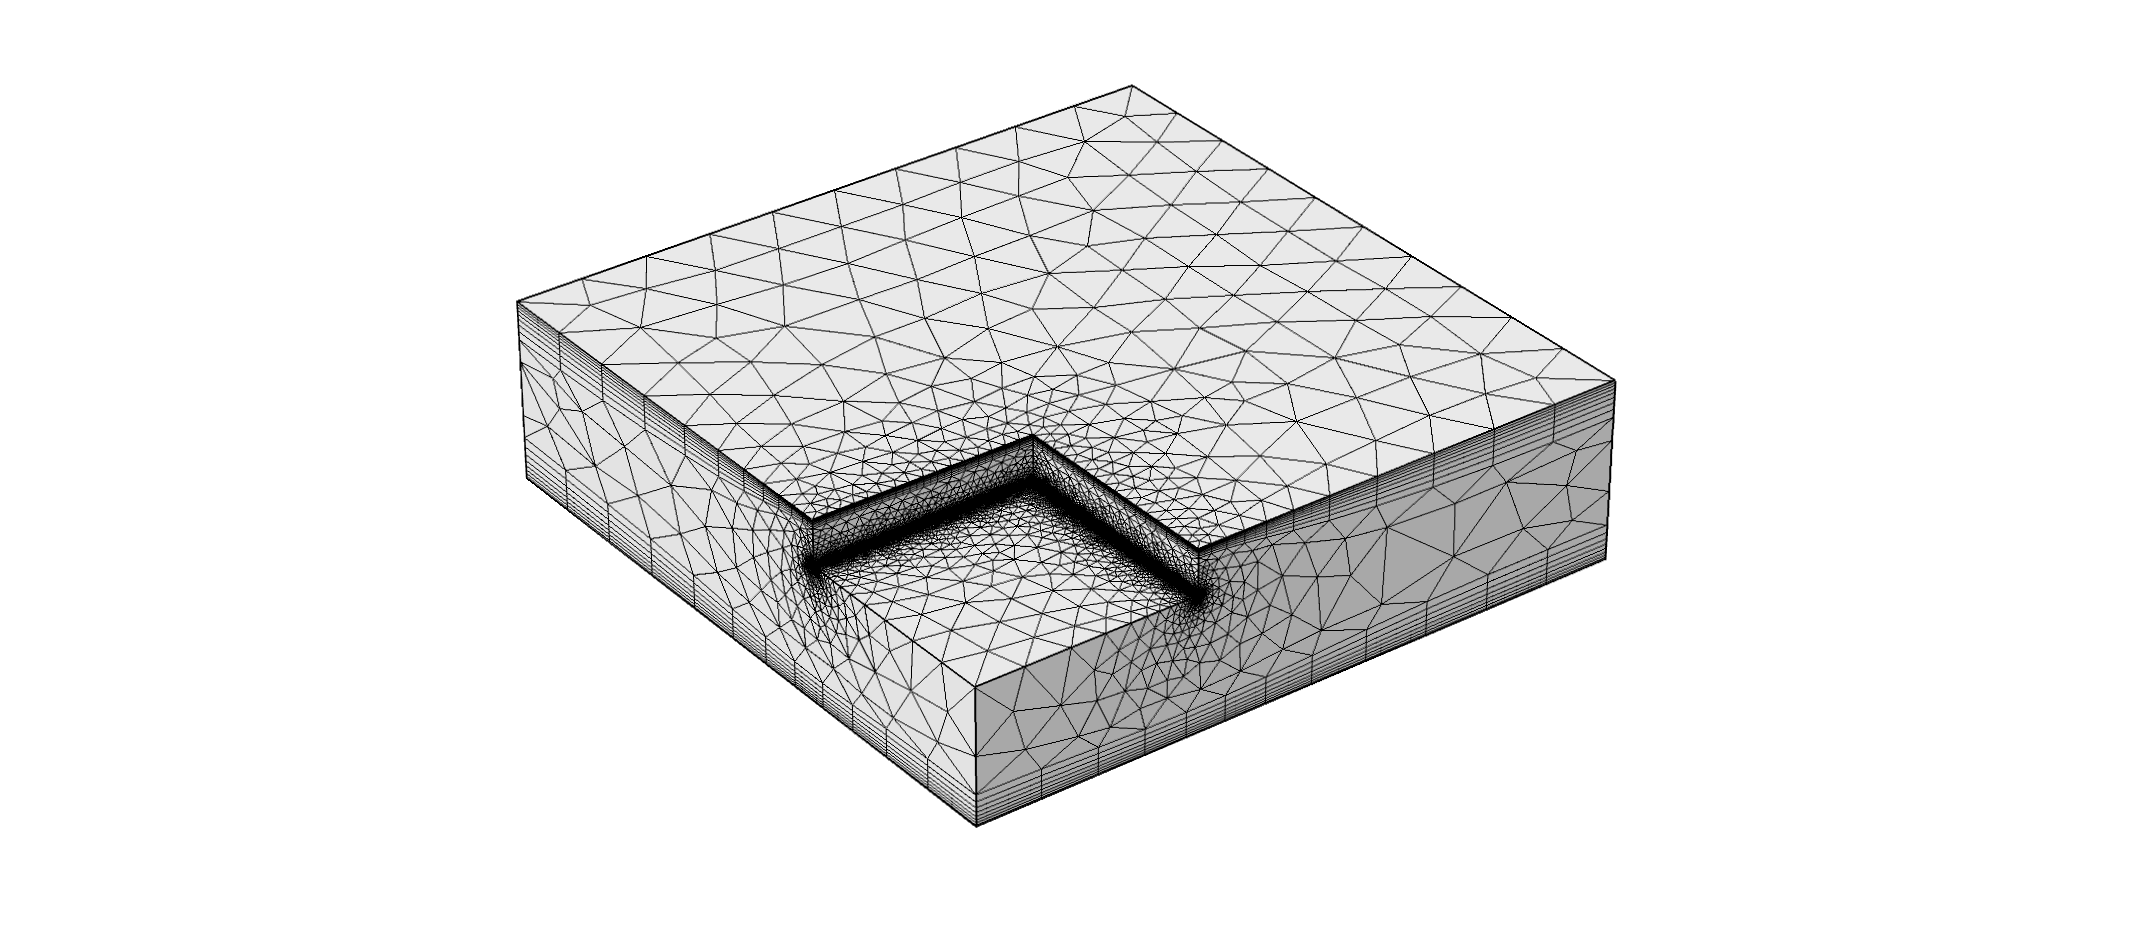
\includegraphics[width=0.75\textwidth]{meshed_model.png}
    \caption{The darker perimeter around the foundation highlights the higher mesh density along the foundation crack.}
    \label{fig:meshed_geometry}
  \end{subfigure}
  \begin{subfigure}[b]{\textwidth}
    \centering
    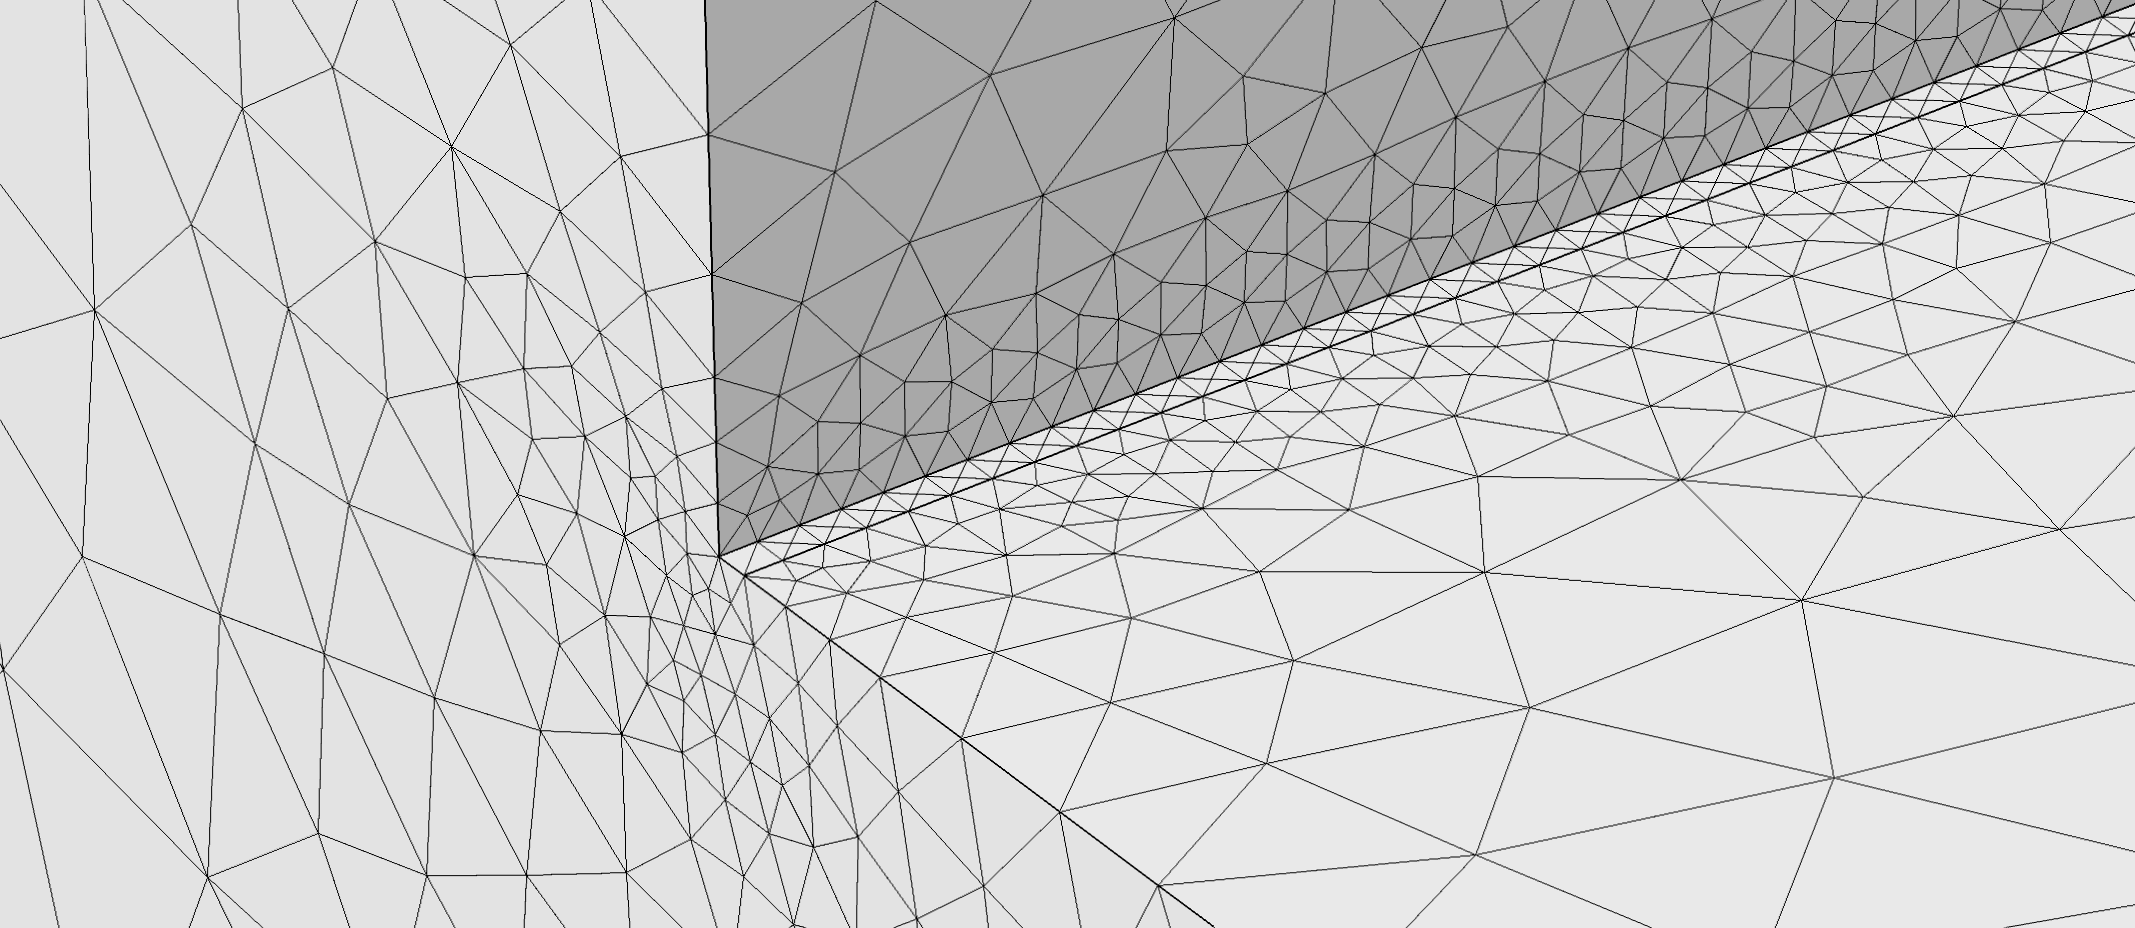
\includegraphics[width=0.75\textwidth]{mesh_crack.png}
    \caption{Close-up of the foundation crack mesh.}
    \label{fig:meshed_crack}
  \end{subfigure}
  \begin{subfigure}[b]{\textwidth}
    \centering
    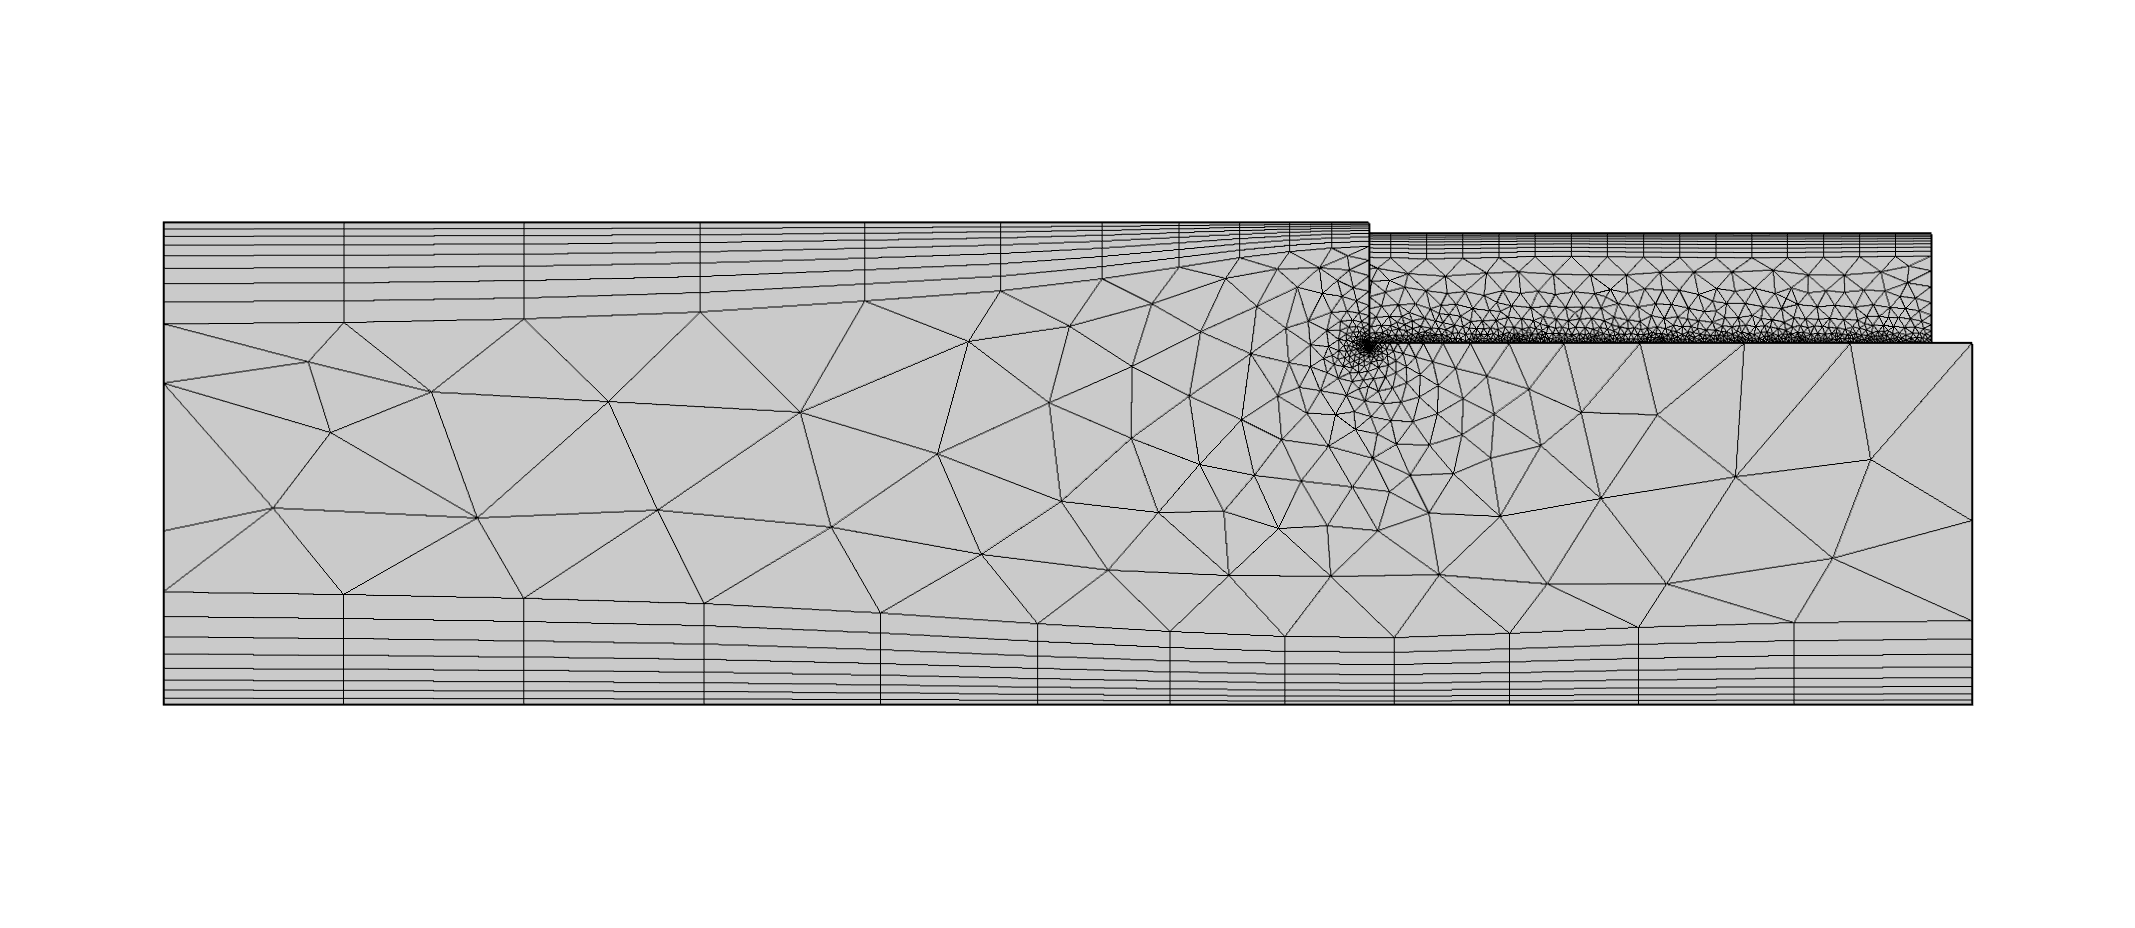
\includegraphics[width=0.75\textwidth]{mesh_boundary_layers.png}
    \caption{Side-view highlighting the boundary layer mesh.}
    \label{fig:mesh_boundary_layers}
  \end{subfigure}
  \caption[Initial finite element mesh of the modeled vapor intrusion scenario.]{Initial finite element mesh of the modeled vapor intrusion scenario.}
  \label{fig:mesh}
\end{figure}
